\documentclass{article}
\usepackage[margin=1in]{geometry}
\usepackage{amsmath}
\usepackage{amssymb}
\usepackage{listings}
\usepackage{color}
\usepackage{titling}
\usepackage[T1]{fontenc}
\usepackage{tcolorbox}
\usepackage{hyperref}
\usepackage{graphicx}
\usepackage{float}

\title{CTF Writeup: \textbf{2024 ICS/IO CTF by Dragos}}
\author{FER tim}

\begin{document}

\begin{center}
    \vspace*{\fill}
    {\LARGE\bf\thetitle}\\[1.5em]
    {\large\theauthor}
    \vspace*{\fill}
\end{center}

\newpage
\tableofcontents
\newpage

\section{Overview}
\label{sec:overview}
Početkom studenog održalo se virtualno Capture the Flag (CTF) natjecanje koje je trajalo 48 sati i 
bilo namijenjeno svima koji se bave ICS/OT sustavima, bez obzira na iskustvo. Sudionici su mogli igrati sami 
ili u timovima te rješavati izazove poput analize phishing e-mailova, PCAP datoteka ICS protokola, Windows logova, 
memorijskih slika, PLC programa i mrežnih dijagrama. Natjecanje je trajalo od 2. do 4. studenog i pružilo priliku za 
istraživanje različitih aspekata OT kibernetičke sigurnosti kroz praktične zadatke.
% ########################################################################################################
% ########################################################################################################
% ########################################################################################################
% ########################################################################################################
% ########################################################################################################
% ########################################################################################################


\section{Digitalna forenzička analiza (\textit{digital forensics analysis})}
\label{sec:forensics}
\subsection{\textit{Arpanet of the Future}}
Zadatak nas upućuje da istražimo Windows Event Viewer log file (.evtx). Uz traženje puno različitih događaja vidimo
da je u jednom trenutku pokrenuta Powershell naredba sa zastavicom -enc koja predstavlja naredbu \textit{encode}.
Defaultno kodiranje je B64 te ako dekodiramo B64 kodirani string koji se nalazi u toj komandi dobijemo flag za ovaj zadatak.
\newline
\newline
\begin{center}
    \textbf{FLAG NIJE OSTAVLJEN}    
\end{center}
\noindent\rule{\textwidth}{0.4pt}

\subsection{\textit{When Are They?}}
SCADA database file se nalazi u \lstinline{/home/operator/.openscada/St.db} i ondje je flag. 
Može se koristiti SQLite ili bilo koji drugi slični program.
\newline
\newline
\begin{center}
    \textbf{FLAG NIJE OSTAVLJEN}    
\end{center}
\noindent\rule{\textwidth}{0.4pt}

\subsection{\textit{De-Loreanize This}}
\begin{tcolorbox}[
    colback=gray!5,  % background color
    colframe=gray!75,  % frame color
    title=\textbf{Zadatak}]
    We caught someone that seemed to be from the past to issue archaic commands at our engineering workstation. Can you figure out what they did?

    Our controller at 10.13.37.37 behaved oddly slow and rebooted once recently.
    
    We only have Powershell Logs … if we only had established monitoring for that controller before….
\end{tcolorbox}

Ponovno kao i prije dobili smo samo .evtx datoteku (loreanized.evtx). Prilikom dekodiranja vidimo sljedeće:
\newline
\begin{lstlisting}[breaklines=true, basicstyle=\ttfamily]
    modbus-send.exe 10.13.37.37 --payload 
    111110101110011111001101110110111100101010111110111111101111110110
    101100001001001111111010110111010110111010011010011011101011001000010
    100111111110100110111010101000110110101111110111011101001111001011010
    010011001100100110001111001101000000100000110001010001100110101010101
    011000000111011010110111011101111111000
\end{lstlisting}

U dekodiranoj datoteci nalazi se tisuće takvih b64 kodiranih linija. Ideja je da se svi ti zapisi spoje u jednu datoteku 
te da se onda iz te datoteke pročita zastavica.

Prije svega valja pretvoriti .evtx datoteku u nekakav čitljivi format. 
Poslužiti ćemo se \url{https://github.com/omerbenamram/evtx} koristeći naredbu:
\lstinline[language=bash]{evtx_dump loreanized.evtx > loreanized.xml}
Sada možemo lako pregledati zapisnike i vidjeti da se poziva \texttt{powershell} s kodiranim naredbama.

Možemo izdvojiti samo kodirane podatke koristeći osnovne alate:
\begin{verbatim}
cat loreanized.xml | grep 'powershell.exe -enc' | uniq | cut -d ' ' -f 3 > base64.txt
\end{verbatim}

Primjer kako se jedna linija ovih kodiranih podataka može dekodirati:
\begin{verbatim}
import base64

line = <kodirani_podatak>
print(base64.b64decode(line).decode('utf-16'))
\end{verbatim}

Dobiveni string može se podijeliti razmacima, a binarni niz može se izdvojiti.

Sljedeći skript dekodira linije, izdvaja binarne nizove i spaja ih u binarnu datoteku:
\begin{verbatim}
import base64

def decode_base64_to_binary(input_file, binary_output_file):
    concatenated_bits = ""

    with open(input_file, 'r') as infile:
        for line in infile:
            line = line.strip()
            decoded_line = base64.b64decode(line).decode('utf-16')
            binary_segment = decoded_line.split()[3]
            concatenated_bits += binary_segment

    with open(binary_output_file, 'wb') as outfile:
        byte_data = int(concatenated_bits, 2).to_bytes((len(concatenated_bits) + 7) // 8, byteorder='big')
        outfile.write(byte_data)

input_file = 'base64.txt'
binary_output_file = 'output.bin'

decode_base64_to_binary(input_file, binary_output_file)
\end{verbatim}

I sada možemo jednostavno pronaći zastavicu:
\begin{verbatim}
strings output.bin | grep flag
\end{verbatim}


\begin{tcolorbox}[
    colback=gray!5,  % background color
    colframe=gray!75,  % frame color
    title=\textbf{Zastavica}]
    \begin{center}
        \textbf{flag\{in\_the\_future\_we\_still\_use\_modbus\}}
    \end{center}
\end{tcolorbox}
\noindent\rule{\textwidth}{0.4pt}

\subsection{\textit{All Se Characters In Installation}}
\begin{tcolorbox}[
    colback=gray!5,  % background color
    colframe=gray!75,  % frame color
    title=\textbf{Zadatak}]
    Someone managed to access our HMI. They popped an MS-Paint screen and weird characters appeared. They did not seem to type it.

Can you help to recover the message?

We managed to get a partial screenshot, but the important part of scrambled. Can you find something in the HMIs memory?

Good thing we have proven technology with XPerienced operators.
\end{tcolorbox}

Nema postupka

\begin{center}
    \textbf{FLAG NIJE OSTAVLJEN}    
\end{center}

\noindent\rule{\textwidth}{0.4pt}

\subsection{\textit{Walking Into A Store And Buying Plutonium}}
\begin{tcolorbox}[
    colback=gray!5,  % background color
    colframe=gray!75,  % frame color
    title=\textbf{Zadatak}]
    We managed to came back to the store with the Finnish operating system and its HMI…its 2022 and the year of the Linux desktop … they now have plutonium in stock, but the HMI has error messages.

    The owner refuses to sell us plutonium until we find the root cause of the error messages.
    
    He managed to capture a screenshot … but it seems manipulated. Luckily he captured a Linux triage package.
\end{tcolorbox}

Nije jasan postupak rješavanja.
\begin{figure}[h]
    \centering
    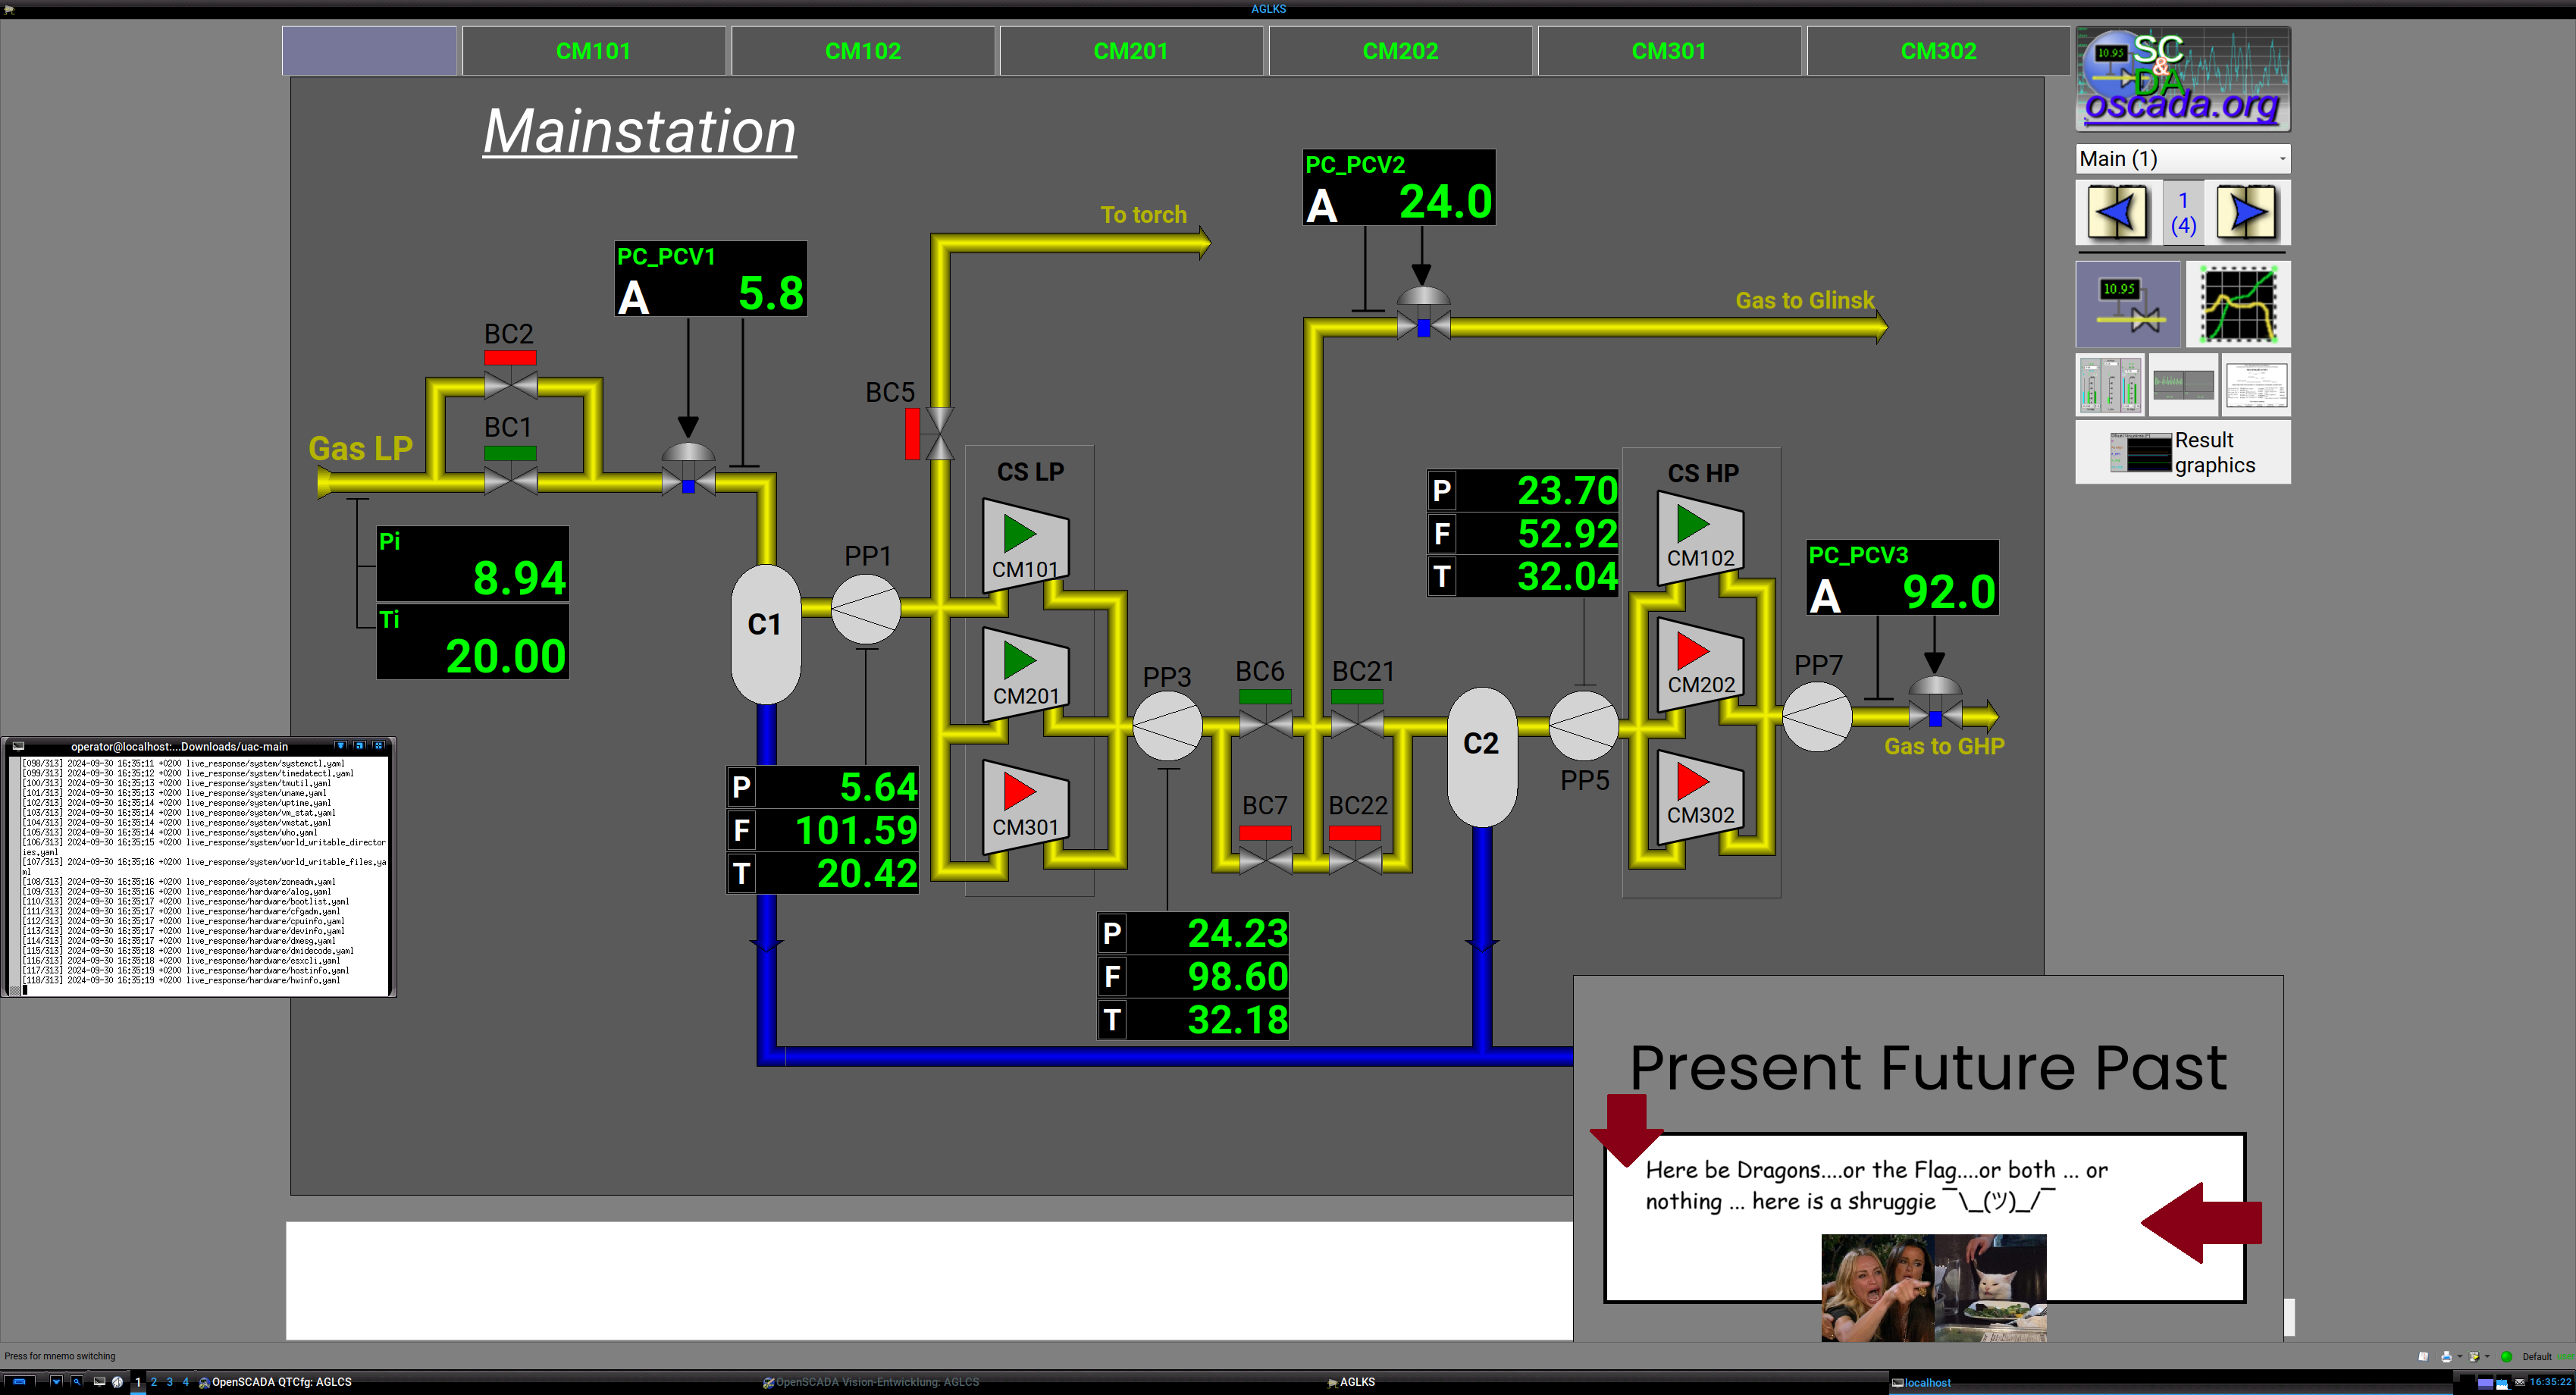
\includegraphics[width=0.8\textwidth]{Walking_Into_a_Store_and_Buying_Plutonium.png}
    \caption{Slika iz zadatka.}
    \label{fig:primjer}
\end{figure}

\begin{center}
    \textbf{FLAG NIJE OSTAVLJEN}    
\end{center}

\noindent\rule{\textwidth}{0.4pt}

% ########################################################################################################
% ########################################################################################################
% ########################################################################################################
% ########################################################################################################
% ########################################################################################################
% ########################################################################################################
% ########################################################################################################
\newpage
\section{Dragos trivia}
\label{sec:trivia}

Ovdje zaista nije potrebno previše govoriti. Dobijemo službene dokumente Dragosa iz kojih je potrebno izvući zastavice.

Zastavice nisu teške te se manje-više brzo pronalaze. Ovaj dio je popularan na svim kompanijskim CTF-ovima jer
imaju priliku podijeliti javno dostupne dokumente te kompanije, točnije podižu svijest o njihovom postojanju.

Možda vam pri pronalaženju pomognu \url{https://youtu.be/babYCpnBbgk?t=1351} ili \url{https://hub.dragos.com/hubfs/Reports/Dragos-FrostyGoop-ICS-Malware-Intel-Brief-0724_r2.pdf?hsLang=en}
\newline
\newline
\begin{center}
    \textbf{Sretno u potrazi :)}
\end{center}
% ########################################################################################################
% ########################################################################################################
% ########################################################################################################
% ########################################################################################################
% ########################################################################################################
% ########################################################################################################
% ########################################################################################################
\newpage
\section{Embedded uređaji}
\label{sec:embedded}
\subsection{\textit{BAD - onBoard Access Device Embedded}}
\begin{tcolorbox}[
    colback=gray!5,  % background color
    colframe=gray!75,  % frame color
    title=\textbf{Zadatak}]
    Zadano je pitanje što se ispisuje na komandnoj liniji kada se sustav pokrene. Uz zadatak dobivamo i ZIP datoteku koja sadrži \texttt{hddimg} datoteku.
\end{tcolorbox}

\begin{itemize}
    \item \textbf{Vrsta datoteke:} \texttt{hddimg} je slika diska, što se potvrđuje korištenjem naredbe \texttt{file}:
    \begin{verbatim}
    BAD.x86.hddimg: DOS/MBR boot sector, code offset 0x58+2, OEM-ID "SYSLINUX", 
    sectors/cluster 4, reserved sectors 4, root entries 512, Media descriptor 
    0xf8, sectors/FAT 212, sectors/track 32, heads 8, sectors 216512 (volumes > 
    32 MB), reserved 0x1, serial number 0xab4cfffc, label: "boot    ", FAT (16 bit)
    \end{verbatim}
    \item Budući da se radi o slici diska, možemo je pokrenuti pomoću QEMU emulatora.
\end{itemize}

Disk slika se pokreće koristeći sljedeću naredbu:
\begin{verbatim}
qemu-system-x86_64 -hda BAD.x86.hddimg -m 2048
\end{verbatim}

\begin{itemize}
    \item Opcija \texttt{-hda} govori QEMU-u da tretira datoteku kao sliku diska.
    \item Opcija \texttt{-m} dodjeljuje 2048 MB RAM-a virtualnom sustavu.
\end{itemize}

\begin{center}
    \textbf{FLAG NIJE OSTAVLJEN}
\end{center}

\noindent\rule{\textwidth}{0.4pt}

\subsection{\textit{BAD Login Challenge}}
\begin{tcolorbox}[
    colback=gray!5,  % background color
    colframe=gray!75,  % frame color
    title=\textbf{Zadatak}]
    Zadano je pitanje što se ispisuje nakon što se prijavimo na uređaj za koji smo dobili sliku diska. Također su nam dani još dva formata iste slike diska: raspberry datotečna slika i OVA slika.
\end{tcolorbox}

\begin{itemize}
    \item \textbf{Vrsta datoteke:} \texttt{hddimg} je slika diska, što se potvrđuje korištenjem naredbe \texttt{file}:
    \begin{verbatim}
    BAD.x86.hddimg: DOS/MBR boot sector, code offset 0x58+2, OEM-ID "SYSLINUX", 
    sectors/cluster 4, reserved sectors 4, root entries 512, Media descriptor 
    0xf8, sectors/FAT 212, sectors/track 32, heads 8, sectors 216512 (volumes > 
    32 MB), reserved 0x1, serial number 0xab4cfffc, label: "boot    ", FAT (16 bit)
    \end{verbatim}
    \item Budući da se radi o slici diska, možemo je pokrenuti pomoću QEMU emulatora.
\end{itemize}

\subsubsection*{Koraci rješenja}
Prvo moramo pristupiti datotekama \texttt{/etc/passwd} i \texttt{/etc/shadow}. Da bismo to postigli, trebamo montirati sliku diska na naš lokalni stroj kako bismo pristupili datotečnom sustavu na disku:
\begin{verbatim}
sudo mkdir /mnt/BAD
sudo mount -o loop BAD.x86.hddimg /mnt/BAD
\end{verbatim}
Ovo će montirati datotečni sustav u direktorij \texttt{/mnt/BAD}. Opcija \texttt{-o loop} je potrebna jer mount očekuje fizički uređaj, a ovo je samo datoteka, pa stvaramo virtualni loopback uređaj.

Ako pogledamo direktorij \texttt{/mnt/BAD}, vidjet ćemo sljedeće datoteke:
\begin{verbatim}
> ls /mnt/BAD
bzImage  EFI  initrd  ldlinux.c32  ldlinux.sys  libcom32.c32  libutil.c32  rootfs.img  startup.nsh  syslinux.cfg  vesamenu.c32
\end{verbatim}
Ovo su tipične datoteke za Linux sustav, a datoteka koja nas zanima je \texttt{rootfs.img}. Ova datoteka sadrži datotečni sustav koji koristi sustav nakon što se pokrene, pa korisnik koji je tamo smješten bit će korisnik koji se očekuje da se prijavi. Budući da je ovo još jedna slika datotečnog sustava, možemo je montirati baš kao i \texttt{.hddimg} datoteku.

\begin{verbatim}
sudo mkdir /mnt/BADrootfs
sudo mount -o loop rootfs.img /mnt/BADrootfs
\end{verbatim}

Kada pogledamo direktorij \texttt{/mnt/BADrootfs}, vidjet ćemo tipičnu Linux strukturu direktorija. Tamo možemo vidjeti datoteke koje tražimo.

Ako pogledamo datoteku \texttt{/etc/shadow}, izgledat će ovako:
\begin{verbatim}
> cat /etc/shadow
root:$5$4RZXNQ5iSvBlGjaJ$54E3xgE5fH2mTX8bho/W9LBHTHmeeQ/NhxpAqcv8Yd1:15069:0:99999:7:::
daemon:*:15069:0:99999:7:::
bin:*:15069:0:99999:7:::
sys:*:15069:0:99999:7:::
sync:*:15069:0:99999:7:::
games:*:15069:0:99999:7:::
man:*:15069:0:99999:7:::
lp:*:15069:0:99999:7:::
mail:*:15069:0:99999:7:::
news:*:15069:0:99999:7:::
uucp:*:15069:0:99999:7:::
proxy:*:15069:0:99999:7:::
www-data:*:15069:0:99999:7:::
backup:*:15069:0:99999:7:::
list:*:15069:0:99999:7:::
irc:*:15069:0:99999:7:::
_apt:*:15069:0:99999:7:::
nobody:*:15069:0:99999:7:::
\end{verbatim}

Iz ovoga možemo vidjeti da postoji root korisnik koji ima SHA256 hashiranu lozinku. Tu lozinku možemo uzeti i pokušati dešifrirati pomoću alata poput \texttt{john the ripper}, no nisam uspio u tome.

Zato možemo iskoristiti drugi trik. Svaka promjena koju napravimo unutar montiranog datotečnog sustava bit će odražena u datoteci iz koje smo montirali datotečni sustav. Dakle, ako promijenimo datoteku \texttt{/etc/shadow} u direktoriju \texttt{/mnt/BADrootfs}, to će biti odraženo u datoteci \texttt{rootfs.img} u direktoriju \texttt{/mnt/BAD}, koja će potom biti odražena u našoj početnoj slici diska \texttt{BAD.x86.hddimg}. Promijenit ćemo datoteku tako da root korisnik nema lozinku. Ovo možemo postići jednostavnim uklanjanjem druge kolone u datoteci, na sljedeći način: \texttt{root::15069:0:99999:7:::}. Ako spremimo ove promjene i odmontiramo oba datotečna sustava pomoću naredbe \texttt{umount}, trebali bismo imati promijenjenu sliku diska u kojoj root korisnik nema lozinku.

\begin{verbatim}
sudo umount /mnt/BADrootfs
sudo umount /mnt/BAD
\end{verbatim}

Da bismo to potvrdili, možemo pokrenuti sliku pomoću QEMU-a:
\begin{verbatim}
qemu-system-x86_64 -hda BAD.x86.hddimg -m 2048
\end{verbatim}

Nakon što slika završi s pokretanjem, jednostavno se prijavite kao root korisnik i primijetit ćete da nema prompta za lozinku, a sustav ispisuje flag.
\begin{center}
    \textbf{FLAG NIJE OSTAVLJEN}
\end{center}

\noindent\rule{\textwidth}{0.4pt}

\subsection{\textit{BAD What Three Words}}
\begin{tcolorbox}[
    colback=gray!5,  % background color
    colframe=gray!75,  % frame color
    title=\textbf{Zadatak}]
    Zadatak traži da brute-forcamo lozinku iz prethodnog zadatka. Također, dobili smo obrazac izgleda lozinke: \texttt{sprink**.fevere*.shoc**}.
\end{tcolorbox}

\subsubsection*{Koraci rješenja}
Za početak, moramo pretvoriti datoteke \texttt{/etc/shadow} i \texttt{/etc/passwd} u format koji \texttt{john} razumije. Naredba za to izgleda ovako:
\begin{verbatim}
unshadow /etc/passwd /etc/shadow > unshadow.txt
\end{verbatim}

Zatim, pokrenimo \texttt{john} s odgovarajućim maskama za brute-forcing:
\begin{verbatim}
john --mask="sprink?l?l.fevere?l?l.shock?l?l" unshadow.txt
\end{verbatim}

Ovdje \texttt{?l} označava da \texttt{john} pokušava bilo koje malo slovo na tom mjestu.

Na mom računaru, ovo je trajalo oko 15 minuta da bi se pronašla točna lozinka: \texttt{sprinkle.fevered.shocks}. Ako ste slučajno očistili terminal ili iz nekog razloga trebate ponovo vidjeti lozinku, možete koristiti sljedeću naredbu:
\begin{verbatim}
john --show unshadow.txt
\end{verbatim}

\begin{center}
    \textbf{FLAG NIJE OSTAVLJEN}
\end{center}

\noindent\rule{\textwidth}{0.4pt}

\subsection{\textit{BAD Unit Test}}
\begin{tcolorbox}[
    colback=gray!5,  % background color
    colframe=gray!75,  % frame color
    title=\textbf{Zadatak}]
    Pronašli smo tri riječi i znamo koje tri riječi imaju sličan format. Sada moramo saznati što se nalazi na toj lokaciji.

    Razvoj ovog računara čini se da potiče iz neobičnog izvora. Još uvijek nismo u mogućnosti prepoznati jezik i moramo se osloniti na geografiju. Guten Tag?

    Možete li pronaći broj jedinice odgovorne za manipulaciju povezanu s tom lokacijom?
    
    \textbf{Format flag-a:} Unit \texttt{NUMBER}
\end{tcolorbox}

\begin{center}
    \textbf{FLAG NIJE OSTAVLJEN}
\end{center}

\noindent\rule{\textwidth}{0.4pt}

\subsection{\textit{BAD XZOR}}
\begin{tcolorbox}[
    colback=gray!5,  % background color
    colframe=gray!75,  % frame color
    title=\textbf{Zadatak}]
    Uspjeli smo obrnuto inženjirati standard za pohranu podataka na BAD uređaju. I to je loše. Možda ste već pronašli zip arhivu na našem firmware imidžu - ako niste, pronađite je. Koristite tri riječi (sve malim slovima, spojene točkama, npr. banana.potato.squirrel) za otključavanje arhive.

    Uspjeli smo identificirati da čini se da nije potreban poseban ključ za dekriptiranje datoteke - sve je tu, čim sustav pokrene.

    Koja je godina… Budućnost, Sadašnjost, Prošlost? Izgubio sam trag. Možda trebamo napraviti korak unatrag.

    Ljubazno podsjećanje da će timovi biti KAZNJENI za savjete na izazovima sa 800 i 1000 bodova!
\end{tcolorbox}
    Prvo, pronađite zip arhivu na firmware slici i otključajte je pomoću tri riječi koje ste dobili (sprinkle.fevered.shocks).

    Zatim, pronađite osnovnu datoteku unutar arhive. Nakon što je pronađete, trebate provesti operaciju XOR na datoteci koristeći njezin vlastiti ključ. To možete postići tako da svaku bajt vrijednost datoteke XORate sa ključem koji je već prisutan u datoteci.

    Kada završite s prvim korakom, datoteku treba dodatno obraditi. Svaki byte osnovne datoteke treba XOR-irati s vrijednošću \texttt{48}. Za ovo ćete vjerojatno koristiti skriptu koja će obraditi sve bajtove.

    Sljedeći korak je učitati rezultat XORanja. Nakon što su svi bajtovi obrađeni, koristite naredbu \texttt{cat} kako biste ispisali datoteku i pregledali sadržaj.

    Ovisno o formatu izlazne datoteke, trebate analizirati sliku ili drugi zapis u kojem će biti ispisan flag. Obratite pažnju na rezultate i uvjerite se da ste ispravno obradili sve bajtove.

    Na kraju, trebali biste moći prepoznati i izdvojiti flag.


\begin{figure}[h]
    \centering
    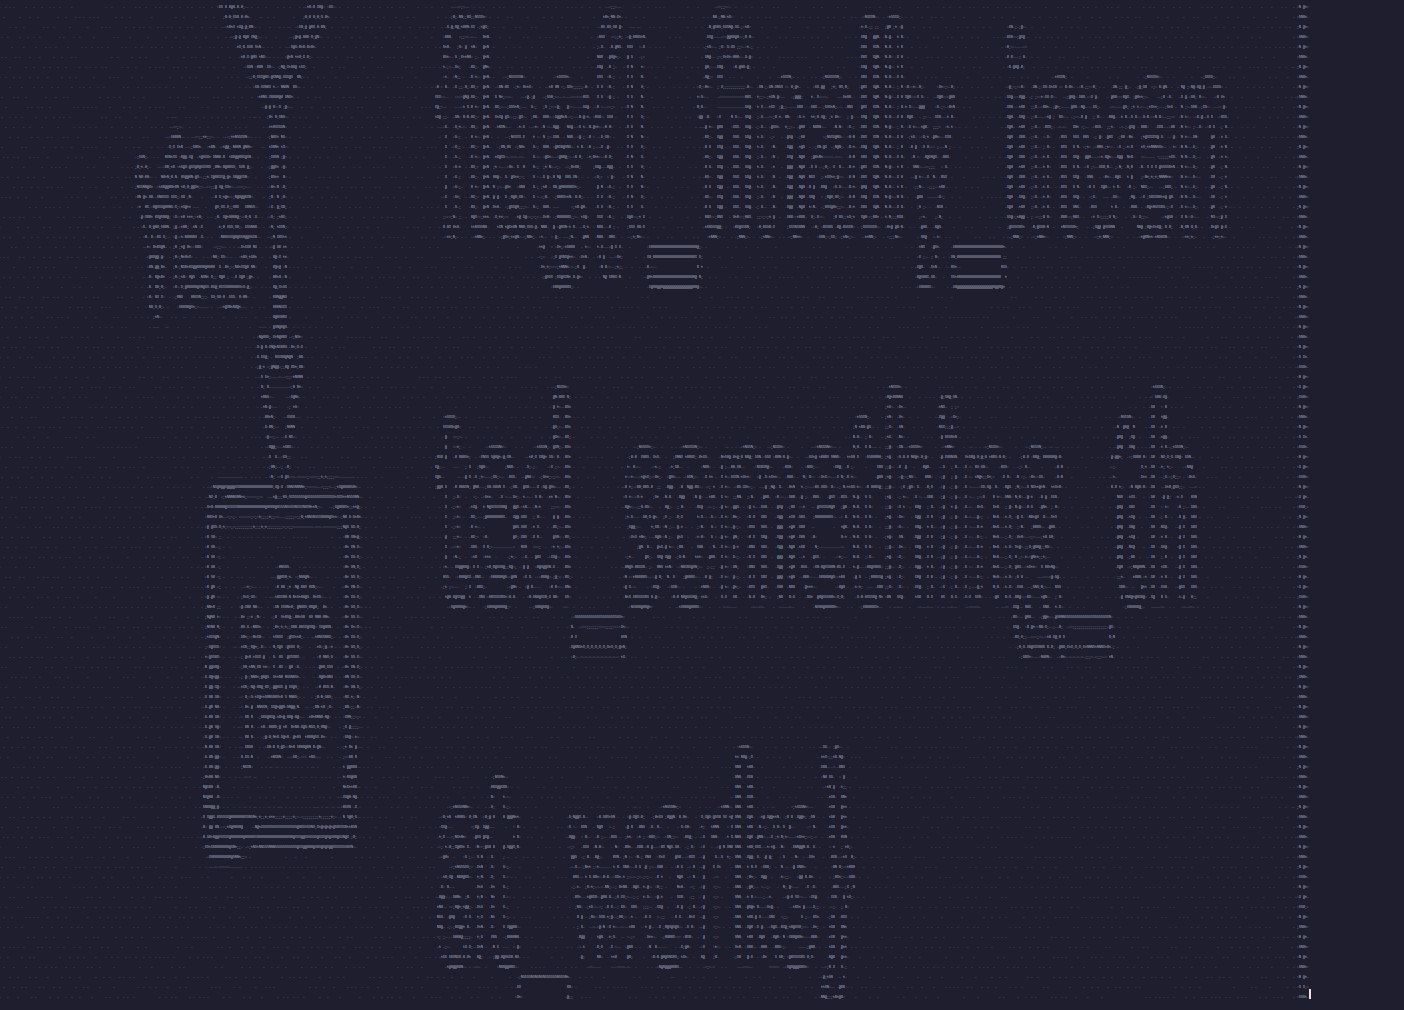
\includegraphics[width=0.8\textwidth]{bad xzor.png}
    \caption{Izgled flaga}
    \label{fig:flag_xzor}
\end{figure}
\noindent\rule{\textwidth}{0.4pt}


% ########################################################################################################
% ########################################################################################################
% ########################################################################################################
% ########################################################################################################
% ########################################################################################################
% ########################################################################################################
% ########################################################################################################
\newpage
\section{Otkrivanje}
\label{sec:discovery}
\subsection{\textit{Something Seems Off Doc}}
\begin{tcolorbox}[
    colback=gray!5,  % background color
    colframe=gray!75,  % frame color
    title=\textbf{Zadatak}]
    Zadana nam je \texttt{pcap} datoteka za analizu kako bismo pronašli ime domaćinskog računala.
\end{tcolorbox}

\begin{itemize}
    \item \textbf{Postupak rješenja:} Budući da ne postoji DNS protokol u prometu, pretpostavljamo da se radi o lokalnoj mreži, pa pokušavamo pronaći \texttt{nbns} (NetBIOS Name Service) protokol.
    \item \textbf{Koraci:} 
    \begin{itemize}
        \item Analizirajte \texttt{pcap} datoteku za pronalazak \texttt{nbns} protokola.
        \item Nakon što pronađemo \texttt{nbns} promet, provjeravamo odgovor na upit za ime.
    \end{itemize}
\end{itemize}

\begin{figure}[h]
    \centering
    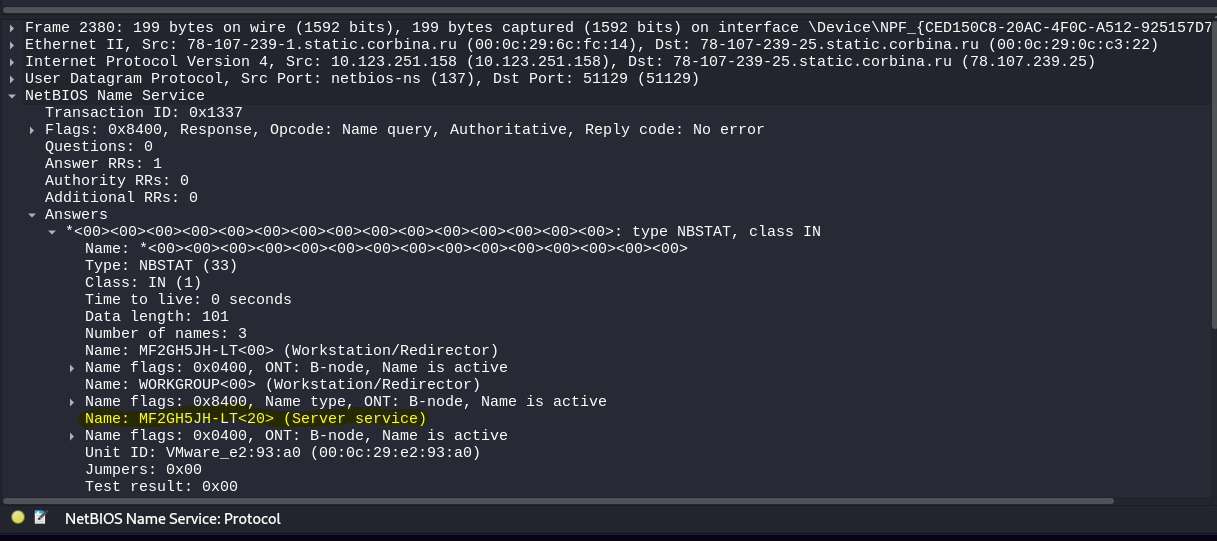
\includegraphics[width=0.8\textwidth]{SomethingSeemsOffDoc.png}
    \caption{Izgled iz Wiresharka}
    \label{fig:flag_ws_doc}
\end{figure}

\begin{center}
    \textbf{MF2GH5JH-LT}
\end{center}

\noindent\rule{\textwidth}{0.4pt}

\subsection{\textit{Where Do We Start?}}
\begin{tcolorbox}[
    colback=gray!5,  % background color
    colframe=gray!75,  % frame color
    title=\textbf{Zadatak}]
    Ovaj zadatak je nastavak analize \texttt{pcap} datoteke iz zadatka "Something Seems Off Doc". Ovdje je cilj pronaći grad povezan s vanjskom IP adresom.
\end{tcolorbox}

\begin{itemize}
    \item \textbf{Postupak rješenja:} Koristimo DNS razlučivanje (name resolution) kako bismo dobili trag koji vodi do grada.
    \item \textbf{Koraci:}
    \begin{itemize}
        \item U Wiresharku uredimo postavke za razlučivanje imena za IP adresu.
        \item Nakon što uredimo postavke, dobivamo dodatne informacije o IP adresi: \texttt{78-107-239-25.static.corbina.ru}.
        \item Korištenjem domene \texttt{.ru} koja je rezervirana za Rusiju, pretražujemo \texttt{corbina} i nalazimo naziv tvrtke čije je sjedište u Moskvi. To je grad koji tražimo.
    \end{itemize}
\end{itemize}

\begin{center}
    \textbf{Grad: Moskva, Rusija}
\end{center}

\noindent\rule{\textwidth}{0.4pt}

\subsection{\textit{Let's Talk About Port Hardening}}
\begin{tcolorbox}[
    colback=gray!5,  % background color
    colframe=gray!75,  % frame color
    title=\textbf{Zadatak}]
    Ovaj zadatak je nastavak zadataka \textit{"Something Seems Off Doc"} i \textit{"Where Do We Start?"}. Napadač je uspio pristupiti korporativnim resursima iskorištavanjem pogrešno konfiguriranog FTP rješenja. Naš zadatak je otkriti koja je aplikacija korištena i koja verzija te aplikacije.
\end{tcolorbox}

\begin{itemize}
    \item \textbf{Postupak rješenja:} Analiziramo FTP protokole kako bismo identificirali aplikaciju.
    \item \textbf{Koraci:}
    \begin{itemize}
        \item Pronalazimo sljedeći odgovor u FTP komunikaciji: \texttt{220}, što označava pozitivnu potvrdu da je poslužitelj spreman prihvatiti nove klijentske veze.
        \item Prema ovom odgovoru zaključujemo da je aplikacija koja se koristi \texttt{FileZilla Server} u verziji 1.8.2.
    \end{itemize}
\end{itemize}

\begin{figure}[h]
    \centering
    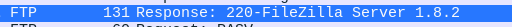
\includegraphics[width=0.8\textwidth]{Let's Talk About Port Hardening.png}
    \caption{Polje paketa u Wiresharku}
    \label{fig:flag_wireshark}
\end{figure}

\begin{center}
    \textbf{Aplikacija: FileZilla Server, Verzija: 1.8.2}
\end{center}

\noindent\rule{\textwidth}{0.4pt}

% ########################################################################################################
% ########################################################################################################
% ########################################################################################################
% ########################################################################################################
% ########################################################################################################
% ########################################################################################################
% ########################################################################################################
\newpage
\section{Prvobitni pristup (\textit{initial access})}
\label{sec:access}
\subsection{\textit{Knocking at the Door}}
\begin{tcolorbox}[
    colback=gray!5,  % background color
    colframe=gray!75,  % frame color
    title=\textbf{Zadatak}]
    Ovaj zadatak je nastavak prethodnih, \textit{"Something Seems Off Doc"}, \textit{"Where Do We Start?"} i \textit{"Let's Talk About Port Hardening"}. Datoteka je preuzeta korištenjem FTP protokola. Naš zadatak je otkriti ime preuzete datoteke.
\end{tcolorbox}

\begin{itemize}
    \item \textbf{Postupak rješenja:} Analiziramo FTP protokole i tražimo naredbu \texttt{RETR} koja se koristi za preuzimanje datoteka.
    \item \textbf{Koraci:}
    \begin{itemize}
        \item Pronalazimo upotrebu \texttt{RETR} naredbe u FTP komunikaciji, što nam pokazuje da je datoteka preuzeta.
        \item Ime preuzete datoteke je \texttt{dontforget.txt}, što je naš odgovor.
    \end{itemize}
\end{itemize}

\begin{center}
    \textbf{Ime datoteke: dontforget.txt}
\end{center}

\noindent\rule{\textwidth}{0.4pt}


\subsection{\textit{Keys to the Kingdom}}
\begin{tcolorbox}[
    colback=gray!5,  % background color
    colframe=gray!75,  % frame color
    title=\textbf{Zadatak}]
    Ovaj zadatak je nastavak prethodnih, \textit{"Something Seems Off Doc"}, \textit{"Where Do We Start?"}, \textit{"Let's Talk About Port Hardening"} i \textit{"Knocking at the Door"}. Preuzeta datoteka sadrži korisničko ime i lozinku. Naš zadatak je pronaći lozinku.
\end{tcolorbox}

\begin{figure}[h]
    \centering
    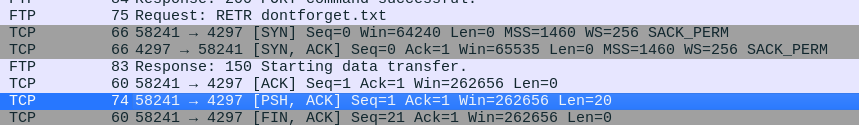
\includegraphics[width=0.8\textwidth]{KeysToKingdom0.png}
    \caption{Paket u Wiresharku}
    \label{fig:pckt_wireshark}
\end{figure}

\begin{figure}[h]
    \centering
    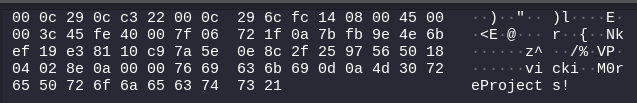
\includegraphics[width=0.8\textwidth]{KeysToKingdom.png}
    \caption{HEX zapis lozinke i korisničkog imena}
    \label{fig:flag_wireshark_Kingdom}
\end{figure}

\begin{itemize}
    \item \textbf{Postupak rješenja:} Analiziramo FTP komunikaciju i gledamo podatke koji su poslani nakon preuzimanja datoteke.
    \item \textbf{Koraci:}
    \begin{itemize}
        \item Nakon što je FTP pozvan, vidimo da je započela prijenos podataka. Odabrani TCP segment ima oznaku \texttt{[PSH, ACK]} i dužinu 20 bajtova, što znači da se podaci nalaze u tom segmentu.
        \item Proučavanjem heksadecimalnog prikaza podataka, možemo vidjeti korisničko ime i lozinku.
        \item Lozinka je \texttt{M0reProjects!}.
    \end{itemize}
\end{itemize}


\begin{center}
    \textbf{Lozinka: M0reProjects!}
\end{center}

\noindent\rule{\textwidth}{0.4pt}

\subsection{\textit{Connecting the Capacitor}}
\begin{tcolorbox}[
    colback=gray!5,  % background color
    colframe=gray!75,  % frame color
    title=\textbf{Zadatak}]
    Svaki put kada povezujemo USB uređaj s Fluxcapacitor-om, pojavljuje se više datoteka nego što smo očekivali. Naš zadatak je pomoći u identificiranju USB uređaja koji je povezan. Sumnjamo da je barem jedan od uređaja prethodno bio korišten na starom industrijskom računalu.
    
    Na kraju, potrebno je pronaći vrijednost \texttt{FriendlyName} USB uređaja.
\end{tcolorbox}

\begin{itemize}
    \item \textbf{Flag format:} Vendor Storage Type (5 Elements separated by spaces).
\end{itemize}
\begin{center}
    \textbf{FLAG NIJE OSTAVLJEN}
\end{center}


\noindent\rule{\textwidth}{0.4pt}


% ########################################################################################################
% ########################################################################################################
% ########################################################################################################
% ########################################################################################################
% ########################################################################################################
% ########################################################################################################
% ########################################################################################################

\newpage
\section{Postojanost (\textit{Persistance})}
\label{sec:persist}
\subsection{\textit{Fluff Capacitor}}
\begin{tcolorbox}[
    colback=gray!5,  % background color
    colframe=gray!75,  % frame color
    title=\textbf{Zadatak}]
    Vjeverice... vjeverice...

    Jedna od tih malih stvorenja uspjela je oštetiti DeLorean. I to ne onako kako biste pomislili... bila je to cyber vjeverica.

    Naš računar je sada pun pahuljastih slika, ali samo je jedna od njih "prava". Koja vjeverica je ona koja nosi monokl, leptir-mašnu, cilindar i puši cigaru, a koja se pojavila u pozadini?

    Uspjeli smo prikupiti sve datoteke sa sustava na daljnju analizu. Neke datoteke na C: su bile "pahuljaste". Umjesto dumpa memorije, dobili smo sistemske datoteke.

    Možemo li prepoznati sliku vjeverice koja je "fluff" i de-fluffati je?
\end{tcolorbox}

\begin{center}
    \textbf{FLAG NIJE OSTAVLJEN}
\end{center}

\noindent\rule{\textwidth}{0.4pt}


\subsection{\textit{We Don't Need No Roads}}
\begin{tcolorbox}[
    colback=gray!5,  % background color
    colframe=gray!75,  % frame color
    title=\textbf{Zadatak}]
    Napomena: Koristite priloženi ZIP za odgovaranje na sljedeća dva pitanja!

    Platili smo skupe usluge za potpuno autonomno putovanje kroz vrijeme, ali još uvijek ne radi. Čini se da nam ipak trebaju ceste da bismo negdje stigli, a naš "pretplata za putovanje kroz vrijeme" izgleda da se može daljinski kontrolirati.

    Sumnjamo da nešto nije u redu nakon posljednjeg posjeta prodavaču automobila. Spomenuli su nešto o ažuriranju firmvera i "nole modu".

    Koje "Ime tvrtke" je odgovorno za probleme s našim DeLoreanom?

    \textbf{Flag Format:} \texttt{flag\{enterthistext\}}

\end{tcolorbox}

\begin{itemize}
    \item Za početak, analizirat ćemo snimku memorije pomoću \texttt{volatility2} (jer \texttt{volatility3} nije radio).
    \item Prvo koristimo \texttt{imageinfo} kako bismo identificirali tip slike memorije:
    \begin{verbatim}
    python2 vol.py -f /path/to/memory/image.vmem imageinfo
    \end{verbatim}
    Ovdje ćemo vidjeti da je slika memorije Windows XP i to ćemo koristiti za daljnje analize.
    
    \item Sljedeći korak je lista svih procesa pomoću \texttt{pslist} komande:
    \begin{verbatim}
    python2 vol.py -f /path/to/memory/image.vmem --profile=WinXPSP2x86 pslist
    \end{verbatim}
    Ovdje ćemo primijetiti sumnjiv proces nazvan \texttt{We don't need no roads.exe}.
    
    \item Za detalje o ovom procesu koristimo \texttt{verinfo} komandu koja će nam otkriti ime tvrtke odgovorne za ovaj proces:
    \begin{verbatim}
    python2 vol.py -f /path/to/memory/image.vmem --profile=WinXPSP2x86 verinfo
    \end{verbatim}
    Iz podataka o verziji pronaći ćemo ime tvrtke.
\end{itemize}

\begin{center}
    \textbf{FLAG NIJE OSTAVLJEN}
\end{center}

\noindent\rule{\textwidth}{0.4pt}

\subsection{\textit{We Don't Need No Roads too}}
\begin{tcolorbox}[
    colback=gray!5,  % background color
    colframe=gray!75,  % frame color
    title=\textbf{Zadatak}]
    DeLorean se ponaša drugačije nego inače. Svaki put kad pokrenemo stroj, svjetla trepere nerazmjerno. Svaki put kad obavimo postupak pokretanja.

    Kad smo istraživali, nismo još pregledali sve registre. Možete li nam pomoći pronaći što točno ometa pokretanje? Znamo da pokreće neki program, ali nemamo ključ za vrijednosti.

    Dijelovi memorije su oštećeni i moramo biti uporni. Ključevi registra su u čudnom jeziku.

    Podsjetnik: Timovi će biti kažnjeni ako uzmu pomoć za izazove s 800 i 1000 bodova!

    \textbf{Flag Format:} Slično normalnim flagovima, ali malo drugačije. Flag ne sadrži heksadecimalne brojeve.

\end{tcolorbox}

\paragraph{Koraci:}

Ovaj zadatak zahtijeva analizu memorijske slike, specifično registar podataka. Koristit ćemo \texttt{volatility} kako bismo pristupili registar podacima i identificirali program odgovoran za ometanje pokretanja.

\begin{itemize}
    \item Prvo, pregledavamo memorijsku sliku pomoću \texttt{hivelist} komande u \texttt{volatility} kako bismo otkrili dostupne registar hives.
    \begin{verbatim}
    python2 vol.py -f /path/to/memory/image.vmem --profile=WinXPSP2x86 hivelist
    \end{verbatim}
    Ovaj korak će identificirati sve registre na sustavu. Ključne stavke su oni koji se odnose na \texttt{NTUSER.DAT} datoteke, što su korisnički registri.

    \item Zatim, istražujemo registar koji se odnosi na \texttt{Run} ključeve, jer ovi ključevi sadrže podatke o programima koji se automatski pokreću prilikom startanja računala. U ovom slučaju, koristimo \texttt{printkey} komandu:
    \begin{verbatim}
    python2 vol.py -f /path/to/memory/image.vmem --profile=WinXPSP2x86 printkey -o 0xe1ce0008 -K "Software\Microsoft\Windows\CurrentVersion\Run"
    \end{verbatim}
    U ovom primjeru, otkrivamo vrijednosti koje nisu ispravno prikazane zbog nepoznatog jezika u registru.

    \item Kako bismo u potpunosti dobili sirove podatke iz registra, koristimo \texttt{dumpregistry} komandu koja izdvaja kompletan registar u datoteku:
    \begin{verbatim}
    python2 vol.py -f /path/to/memory/image.vmem --profile=WinXPSP2x86 dumpregistry --dump-dir regdump
    \end{verbatim}
    Ova komanda izdvaja registar u datoteku koju možemo istraživati.

    \item Zatim možemo koristiti alat kao što je \texttt{hivex} za analizu registrirane datoteke:
    \begin{verbatim}
    hivexsh registry.0xe1ce0008.NTUSERDAT.reg
    \end{verbatim}
    U ovom alatu, izdvajamo vrijednosti ključeva pomoću \texttt{lsval} komande da bismo dobili vrijednost nepoznatog ključa, koja nam otkriva naziv programa koji je odgovoran za problem.

\end{itemize}

\begin{center}
    \textbf{flag\{DeLorean\}}
\end{center}
\noindent\rule{\textwidth}{0.4pt}
% ########################################################################################################
% ########################################################################################################
% ########################################################################################################
% ########################################################################################################
% ########################################################################################################
% ########################################################################################################
% ########################################################################################################
\newpage
\section{Analiza ICS protokola}
\label{sec:access}
\subsection{\textit{Doc's Mysterious Transmission}}
\begin{tcolorbox}[
    colback=gray!5,  % background color
    colframe=gray!75,  % frame color
    title=\textbf{Zadatak}]
    Dok je čistio garažu, Marty McFly je naišao na stari računar s tajanstvenom porukom od Doc-a, datiranu na 26. listopad 1985. Poruka se čini da se odnosi na kontrolni sustav za DeLoreansov flux capacitor, ali završava naglo.

    Analiziraj priloženi PCAP fajl, koji sadrži mrežni promet snimljen s Doc-ovog računara. Tvoj zadatak je dekodirati transmisiju i dohvatiti tajnu frazu koju je Doc koristio za aktiviranje flux capacitor-a.

    Koja je tajna fraza?
\end{tcolorbox}

\begin{center}
    \textbf{FLAG NIJE OSTAVLJEN}
\end{center}
\noindent\rule{\textwidth}{0.4pt}

\subsection{\textit{Temporal Network Anomaly}}
\begin{tcolorbox}[
    colback=gray!5,  % background color
    colframe=gray!75,  % frame color
    title=\textbf{Zadatak}]
    Doc-ov posljednji eksperiment uključuje slanje podataka unazad kroz vrijeme. PCAP fajl s ovog eksperimenta pokazuje čudne uzorke i anomalije koje bi potencijalno mogle otkriti tajne putovanja kroz vrijeme.

    Analiziraj priloženi PCAP fajl kako bi razumio prirodu vremenskih anomalija. Tvoj cilj je odrediti točan trenutak u podacima kada se vremenska distorzija dogodila.

    Možeš li prepoznati budući datum?
\end{tcolorbox}

\paragraph{Način Rješavanja}:
Da bismo riješili ovaj zadatak, analizirali smo PCAP fajl i primijetili funkciju koja čita vrijeme. Ova funkcija je pozvana četiri puta, a tri puta se odnosi na godinu 2014. Samo je jedan poziv imao datum iz 2034. godine, što ukazuje na to da je ta vrijednost anomalija iz budućnosti. Ova anomalija je ključna za odgovor na pitanje.

\begin{figure}[h]
    \centering
    
\includegraphics[width=0.8\textwidth]{TemporalNetAnom.png}
    \caption{Flag}
    \label{fig:flag_wireshark_temporal}
\end{figure}

\begin{center}
    \textbf{Aug 20, 2034 00:00:00.000}
\end{center}

\noindent\rule{\textwidth}{0.4pt}

\subsection{\textit{Emmet's Energy Puzzle}}
\begin{tcolorbox}[
    colback=gray!5,  % background color
    colframe=gray!75,  % frame color
    title=\textbf{Zadatak}]
    Imamo pcap fajl u kojem je promijenjena vrijednost. Naša zadaća je analizirati podatke, razumjeti promjenu i otkriti sustav u kojem je vrijednost promijenjena. Znamo da je za Doc-ovo putovanje potrebna energija od 1.21GW.

    Tvoj zadatak je pronaći anomaliju i točan sustav u kojem je vrijednost promijenjena.
\end{tcolorbox}

\paragraph{Način Rješavanja}: 
Za rješenje ovog zadatka otvorili smo pcap fajl u Wiresharku i koristili opciju "Follow TCP Stream" kako bismo pregledali podatke iz razgovora. Podaci su bili šifrirani u base64 formatu, pa smo ih dekodirali kako bi postali čitljivi. Nakon dekodiranja podataka, otkrili smo da je vrijednost potrebne energije postavljena na 3.21GW unutar sustava \texttt{DeLoreanPowerSystem.EnergyDistribution.TimeTravelCircuits}. Ovaj sustav je bio odgovoran za promjenu vrijednosti.

\begin{center}
    \textbf{DeLoreanPowerSystem.EnergyDistribution.TimeTravelCircuits}
\end{center}

\noindent\rule{\textwidth}{0.4pt}

\subsection{\textit{The Biff Tannen Override}}
\begin{tcolorbox}[
    colback=gray!5,  % background color
    colframe=gray!75,  % frame color
    title=\textbf{Zadatak}]
    Biffovi prijatelji uspjeli su infiltrirati sustav za upravljanje prometom u Hill Valleyu. Ostavili su konfiguracijsku datoteku na mreži koja može manipulirati semaforima u gradu, uzrokujući nered. Imate pristup snimci prometa s ovog sustava. Vaš zadatak je razumjeti Biffove naredbe za preuzimanje kontrole i vratiti normalno stanje prometa.

    Koje je ime jedne od glavnih ulica koje je Biff izmijenio?
\end{tcolorbox}

\paragraph{Način Rješavanja}:
Za rješenje zadatka koristili smo dva streama podataka: \texttt{xdata.txt} i \texttt{xdata\_s.txt}. Prva IP adresa bila je označena kao 1.20, a druga kao 1.30. Koristio sam XOR operaciju za usporedbu oba streama (\texttt{xdata} i \texttt{xdata\_s}) i za svaki bit primijenio XOR s vrijednošću \texttt{01111001}. Nakon izvođenja XOR operacija, mogli smo dešifrirati informacije koje su sadržavale ime glavne ulice koju je Biff modificirao.

\begin{center}
    \textbf{FLAG NIJE OSTAVLJEN}
\end{center}

\noindent\rule{\textwidth}{0.4pt}

\subsection{\textit{Save the Clock Tower Hack}}
\begin{tcolorbox}[
    colback=gray!5,  % background color
    colframe=gray!75,  % frame color
    title=\textbf{Zadatak}]
    Identificirana prijetnja, Biffovi prijatelji, ciljali su sat na zvoniku u Hill Valleyu, pokušavajući promijeniti rad električnog motora koji podiže utege sata. Srećom, pristup sustavu za kontrolu motora je nadgledan, a snimke mrežnog prometa su dostupne.

    Triage tim nije pronašao ništa zlonamjerno u PCAP-ovima, ali Dragos Intelligence tim je pružio dodatne uvide koji bi trebali biti pregledani detaljnije. Čini se da Biffovi prijatelji obično kradu inženjerske specifikacije prije nego što pokušaju manipulirati kontrolnim sustavom.
\end{tcolorbox}

\begin{figure}[H]
    \centering
    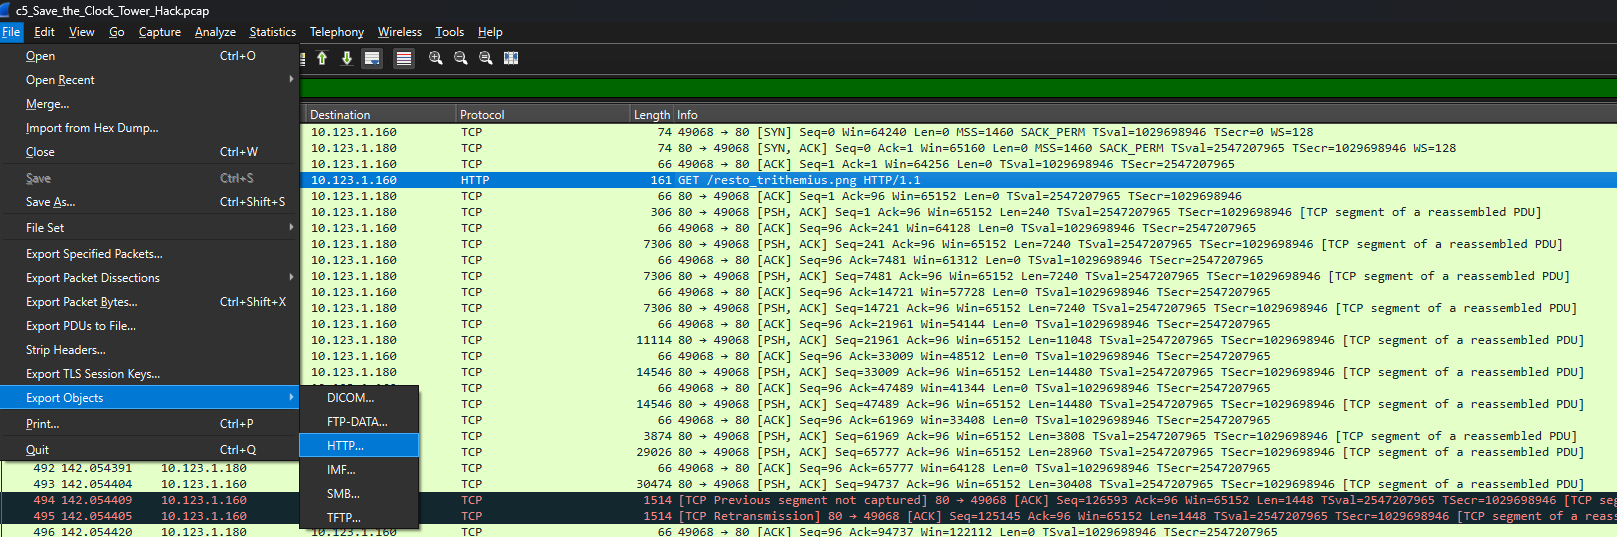
\includegraphics[width=0.8\textwidth]{wiresharkClock.png}
    \caption{Paket u Wiresharku}
    \label{fig:pckt_wireshark_Clock}
\end{figure}

\paragraph{Način Rješavanja}
Iz PCAP datoteke izvukli smo sliku, koju smo zatim obradili pomoću online alata \href{https://www.aperisolve.com/}{AperiSolve}. Rezultat obrade je bio rješenje:

\begin{figure}[H]
    \centering
    \begin{minipage}{0.5\textwidth}
        \centering
        
\includegraphics[width=\linewidth]{resto_trithemius.png}
        \caption{Orginalna slika}
        \label{fig:orginalna}
    \end{minipage}%
    \begin{minipage}{0.5\textwidth}
        \centering
        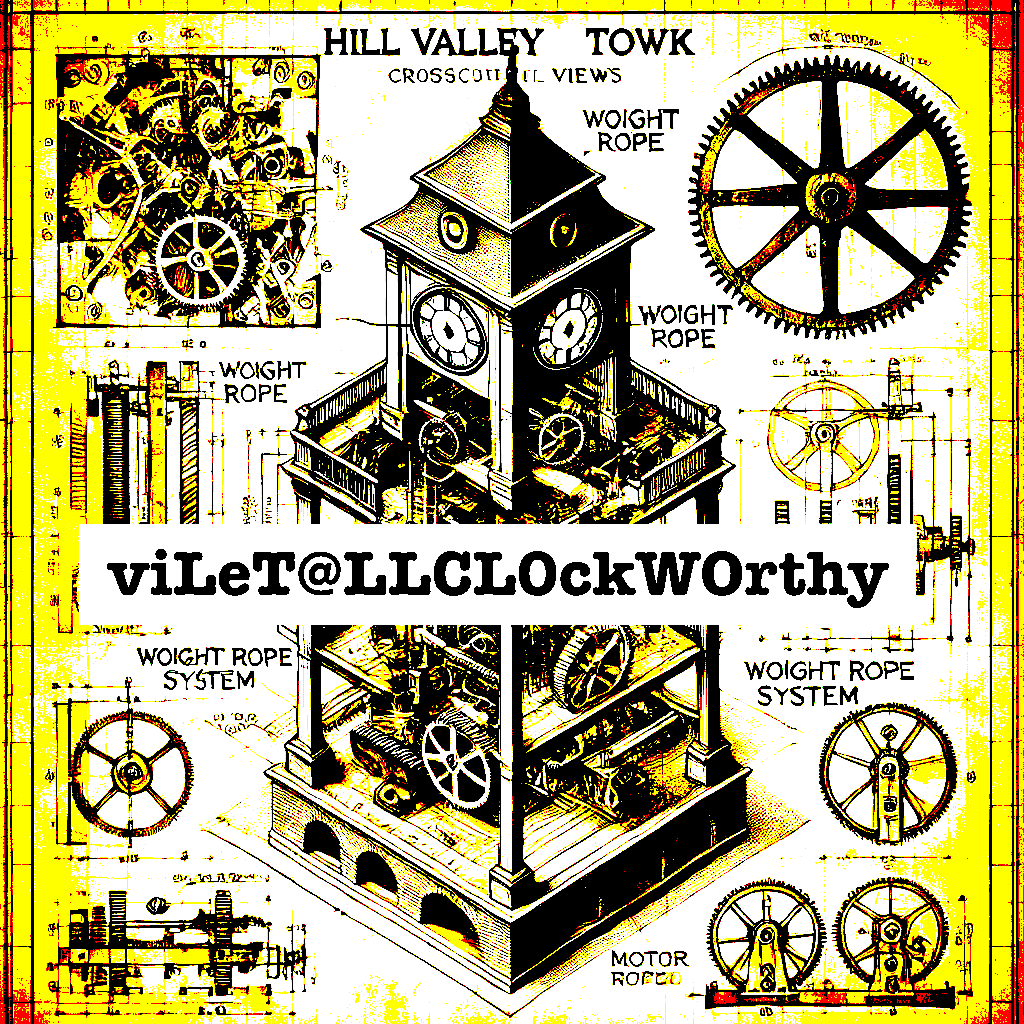
\includegraphics[width=\linewidth]{image_rgb_1.png}
        \caption{Filtrirana slika}
        \label{fig:filtrirana}
    \end{minipage}
\end{figure}

\begin{center}
    \textbf{viLeT@LLCLOckWOrthy}
\end{center}

\noindent\rule{\textwidth}{0.4pt}

\subsection{\textit{Operation Lights Out}}
\begin{tcolorbox}[
    colback=gray!5,  % background color
    colframe=gray!75,  % frame color
    title=\textbf{Zadatak}]
    A mysterious malfunction has occurred within Hill Valley's traffic light control system, causing widespread confusion and traffic jams. Preliminary investigations suggest that someone has tampered with the communication between the master control unit and individual traffic light controllers. A PCAP file containing the network traffic during the incident is the only clue available.

    General Instructions for the Player: Examine the provided PCAP file to trace the source and nature of the anomalies in the communication between the master control and the traffic lights. Your objective is to determine the changes made and identify any unusual patterns or commands that could explain the disruptions.

    Flag: The flag is a mysterious command and a message. YOU MUST BUILD THE WHOLE COMMAND (not just the payload!) … but don’t include lower layers info (e.g., Ethernet, IP, or TCP/UDP data). Submit the flag as a hex string representation without any delimiter:

    AABBCCDDEEFF...

    NOTE: Both lowercase and uppercase hex are accepted.

    \textbf{Free hints:}
    \begin{itemize}
        \item Use the .lua
        \item Industrial protocols usually have some well-defined structure (header, command, payload, checksum)
        \item Industrial protocols are usually the payload of other layers \(ethernet/ip/tcp|udp/ind_protocol\).
        \item Just because you don't see a command in a capture, it doesn't mean it doesn't exist.
    \end{itemize}
\end{tcolorbox}

\paragraph{Način Rješavanja}
Prvo smo analizirali PCAP datoteku kako bismo pronašli ključne informacije. Izdvojili smo dvije stavke:
\begin{itemize}
    \item \textbf{Lozinku:} \texttt{GR3@t\_Sc0tT\_M@Rt1}
    \item \textbf{Binary zip arhivu:} koja je bila kodirana u podatkovnom streamu.
\end{itemize}

Potom smo koristili alat \texttt{xxd} za pretvaranje binarnog streama u zip arhivu. Kada smo arhivu raspakirali koristeći pripadajuću lozinku, dobili smo sliku. Na slici je bila prikazana komanda i poruka potrebna za generiranje završnog zahtjeva (flaga).

\begin{figure}[H]
    \centering
    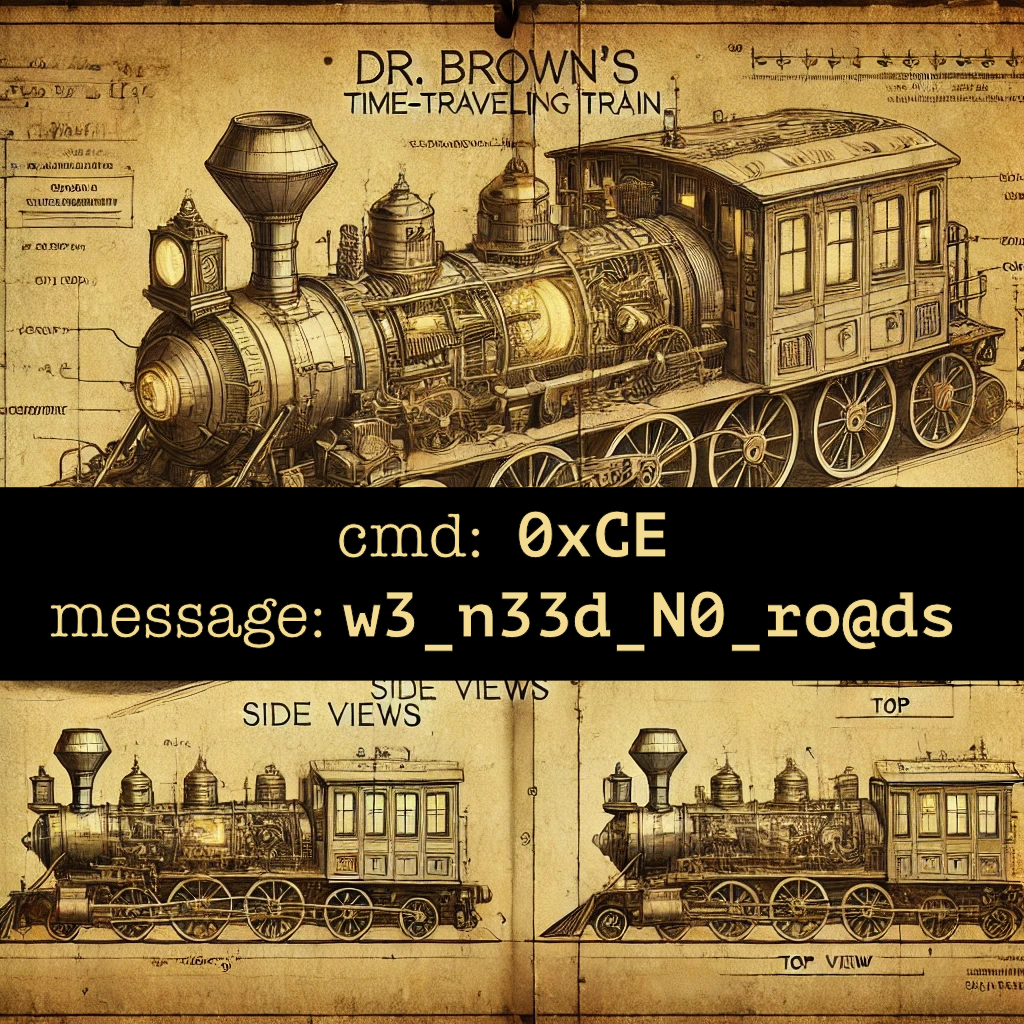
\includegraphics[width=0.8\textwidth]{tlcp_firmware.png}
    \caption{Paket u Wiresharku}
    \label{fig:lights_out}
\end{figure}

Na temelju analize i primjera strukture datagrama HVLTP-a (Hill Valley Traffic Light Protocol), definirali smo paket kako slijedi:
\begin{verbatim}
magic.hvltpVer.requestOrResponse.command.length(1byte-2HEXchrs).message.checksum(2bytes-4HEXchars)
\end{verbatim}

Primjer skripte za dešifriranje HVLTP protokola:
\begin{verbatim}
hvtlp = Proto("HVTLP", "Hill Valley Traffic Light")

-- observed commands
local COMMANDS = {
    [0x10] = "ID",
    [0x11] = "Address",
    [0x12] = "Status",
    [0x14] = "Durations"
}

hvtlp.fields.magic = ProtoField.string("hvtlp.magic", "Magic")
hvtlp.fields.version = ProtoField.uint8("hvtlp.version", "Version")
hvtlp.fields.type = ProtoField.uint8("hvtlp.type", "Type", base.DEC, {[1] = "Request", [2] = "Response"})
hvtlp.fields.command = ProtoField.uint8("hvtlp.command", "Control Code", base.HEX, COMMANDS)

function hvtlp.dissector(buffer, pinfo, tree)

    if (buffer:len() < 10) then return end

    local magic = buffer(0,5):string()
    if magic ~= "1.2GW" then return end

    local request = buffer(6,1):uint()
    local cmd = buffer(7,1):uint()

    pinfo.cols.protocol = hvtlp.name
    local subtree = tree:add(hvtlp, buffer(), "Hill Valley Traffic Light")
    subtree:add(hvtlp.fields.magic, buffer(0,5))
    subtree:add(hvtlp.fields.version, buffer(5,1))
    subtree:add(hvtlp.fields.type, buffer(6,1))
    subtree:add(hvtlp.fields.command, buffer(7,1))

    if COMMANDS[cmd] ~= nil then
        pinfo.cols.info = COMMANDS[cmd] .. " " .. (request == 1 and "Request" or "Response")
    else
        pinfo.cols.info = string.format("Unknown cmd [%02x] ", cmd) .. (request == 1 and "Request" or "Response")
    end

end

tcp_table = DissectorTable.get("tcp.port"):add(54321, hvtlp)
\end{verbatim}

Na temelju ove strukture kreirali smo naš flag, pazeći da dodamo nule na kraju za checksum. Konačni flag u HEX formatu je:

\begin{center}
    \textbf{312e3247570102ce002477335f6e3333645f4e305f726f4064730000}
\end{center}

\noindent\rule{\textwidth}{0.4pt}


% ########################################################################################################
% ########################################################################################################
% ########################################################################################################
% ########################################################################################################
% ########################################################################################################
% ########################################################################################################
% ########################################################################################################
\newpage
\section{Kontrola (\textit{Command and control})}
\label{sec:control}
\subsection{\textit{Botnet Binary of the Future}}
\begin{tcolorbox}[
    colback=gray!5,  % background color
    colframe=gray!75,  % frame color
    title=\textbf{Zadatak}]
    Uspjeli smo doći do uzorka. Ovaj put ga nemamo u memoriji, već je izvađen s jednog od USB uređaja povezanih s plutonijem za fluxcapacitor.

    Pronašli smo nekoliko P1 centrifugnih planova koji su zanimljivi, ali ne čine se povezani s binarnom datotekom - ili možda jesu?

    U svakom slučaju, možeš li saznati koji IOCs (indikatori kompromitacije) možemo koristiti? Čuo sam da su tagovi relevantni za OT komponente.

    Lozinka za zip: infected
\end{tcolorbox}

\begin{center}
    \textbf{FLAG NIJE PRONAĐEN}
\end{center}

% ########################################################################################################
% ########################################################################################################
% ########################################################################################################
% ########################################################################################################
% ########################################################################################################
% ########################################################################################################
% ########################################################################################################
\section{Reversing}
\label{sec:reversing}
\subsection{\textit{Pastastrophe}}
\begin{tcolorbox}[
    colback=gray!5,  % background color
    colframe=gray!75,  % frame color
    title=\textbf{Zadatak}]
    Ažurirani program upravljanja promjenama je nešto što bi svaka organizacija trebala implementirati kako bi osigurala prijenos znanja... ali nisu sve organizacije to učinile...

    I evo nas, prethodni PLC inženjeri su otišli i ostavili malo ili nimalo dokumentacije. Interni tim pokušava dohvatiti vjerodajnice, ali nemaju sreće. Ne znaju lozinku za ovaj nepoznati uređaj.

    Možete li izvući lozinku?

    \textbf{Napomena:} Timovi će biti kažnjeni za korištenje savjeta u izazovima od 800 i 1000 bodova!
\end{tcolorbox}

\begin{center}
    \textbf{FLAG NIJE PRONAĐEN}
\end{center}

\newpage
\section{Zahvale}
\begin{center}
    \vspace*{\fill}
    Zahvaljujem se svima na sudjelovanju u ICS/IO CTFu by Dragos. Čestitam nama na dobrim rezultatima!

    Posebne zahvale:
    prof. dr. sc. Stjepan Groš
    \newline
    mag. ing. Filip Katulić
    \vspace*{\fill}
\end{center}

\end{document}